\nomenclature[]{UE4}{Unreal Engine 4}
\nomenclature[]{RAV}{Robotic Aerial Vehicle}

\subsection{Evaluation Criteria}\label{subsec:EvalCriteria}
In order to design the virtual environment, it was important to first identify the criteria that would determine its usefulness. We began by identifying key physical phenomena that would need to be present, or integrated in future iterations. This was based on an operational scenario that was outlined in the ROCSAFE \href{https://www.nuigalway.ie/rocsafe/research/}{Deliverable 2.4: Detailed Use Cases}\footnote{\href {https://www.nuigalway.ie/rocsafe/research/}{https://www.nuigalway.ie/rocsafe/research/}}. We modelled Use Case 1, with a brief description as follows:\par
"\textit{The scene is set in a rural location, with some forest, a twin track rail line, a small town 10Km away with a small road running near to the rail tracks with access to the rail tracks. The conditions are cool and dry, with a light breeze. A train has been derailed and heavy machinery has been used to damage the tracks. Radioactive material in containers has been exposed. It is intended to use autonomous aerial and ground vehicles to remotely survey and document the scene. They will then be used to localize forensic evidence, subsequently leading to remote evidence collection.}".\par
The result of modelling this scenario using UE4 is shown in Figures \ref{fig:finalVirtualEnv1} and \ref{fig:finalVirtualEnv2}.
%Should talk about the rad. environment here but not sure of dissemination status.


\par In relation to the research question stated above, we identified the most salient data used in hazardous scene management and how it can be realistically generated: 
\begin{itemize}
    \item ROCSAFE and other CBNR scene management reference manuals frequently state the value of a visual overview of the scene \cite{StandardizationOffice2012AJP-3.8ADefence}. In order to generate realistic simulated images, the simulation will need to have high-resolution rendering capabilities.
    \item Further to the above point, the images will need to be generated from the perspective of a RAV in order to be of use when prototyping object detection modules and other AI systems related to ROCSAFE.% This is a key aspect of the ROCSAFE project.
    \item The scene will need to have a configurable physical layout so that occlusion, shadows and other real-world aspects will be present in images. A non-uniform topography is also important for planning potential paths to sources of evidence for sampling.
    \item For the scene described above, a sensor which can simulate radiation readings is necessary, which will record noisy readings that are affected by real-world phenomena such as occlusion.
    \item All data must have timestamps and spatial information associated with it. The spatial information should use a real-world coordinate reference system, such as GPS.
\end{itemize}

%The core components that the simulation of this scenario required were identified and we describe them in terms of evaluation criteria as follows:
We used the above points to discern some technical requirements that the simulation environment would need to achieve, which form our evaluation criteria:
%\note{This is probably the most important part of this chapter}
\begin{itemize}
    \item The ability to place arbitrary realistic virtual representations of physical objects in the scenario in various configurations.
    \item The ability to render high-quality images from the scenario from arbitrary locations at arbitrary resolutions, with common visual phenomena present, such as shadows and lens flare.
    \item There must be sufficient detail in the scene to introduce some noise to image processing problems. This means avoiding a highly-uniform configuration.
    \item Multiple heterogeneous simulated aerial vehicles, with a high-level API for sensing and navigation for each vehicle. The API should not be platform-specific so that different types of vehicle may be considered.
    \item Simulated sensor readings from the aerial vehicles, including position, velocity, altitude, that depend on the state of the aerial vehicle in the environment. For example, if the aerial vehicle is close to a source of radiation, the simulated sensor reading should be high.
    \item Simulation software should have a permissive licence and should permit publications that include details of the software.
    \item The ability to run the simulations at an increased speed without corrupting the fidelity of the sensor/actuator functionality.
    \item The ability to quickly change the configuration of the simulation.
\end{itemize}
\note{More can be added to this list.}

\subsection{Existing Tools and Software}
In order to provide this functionality, it is clear that using existing tools would be desirable, as writing low-level code for tasks such as rendering would take a prohibitive amount of time. Game engines have been increasingly used for simulations of physical phenomena, with a growing interest in niche areas. Examples include generating high-fidelity training data for computer vision algorithms, \cite{Qiu2016UnrealCV:Engine}, deep learning algorithms \cite{Gaidon2016VirtualAnalysis}, automated crowd size estimation algorithms \cite{Lee2018DigitalCrowds} and target tracking algorithms \cite{Mueller2016ATracking}. An overview of literature related to the use of game engines in creating simulation software is outlined in Section \ref{subsec:GameEngineReview}. The overview describes how most modern simulation softwares that use game engine components are mature in their capabilities to model and render physical scenarios, but not all provide good support for the use of robotic vehicles.
%\note{want to get across that basic rendering etc. is offered by many platforms, real issue is to find something to work with that can provide support for Remotely Operated Vehicles / Autonomous vehicles}
This meant that an emphasis was placed on choosing software with some capability to implement high-fidelity simulated aerial vehicles as well as physics and graphics rendering.
%Specific functionality can commonly be added to games engines using plugins, which are usually specific to an individual games engine. 
Standalone simulation tools were considered alongside tools designed to be run using a game engine. The simulation software whose potential use for designing a custom simulation environment for disaster scene management that were investigated are shown in Table \ref{table:SimulatorComparison}, with more detailed overviews provided in \cite{Ebeid2018ASimulators}. UE4, combined with the Airsim plugin, was chosen to develop the simulation since the documentation for both suggested that it could meet all of the the evaluation criteria outlined above. We give more details of the integration of AirSim in Section \ref{sec:AirSimIntegration}.\par
%\note{Might be better off presenting this as a table.
%Format could be Simulator | Licence | Implementation Language | Supported OS | %Developer | Additional Notes}
%\begin{itemize}
%Provide a brief description of each.
%    \item Gazebo: A free, open-source standalone simulator written in C++. Development began at the University of Southern California, now maintained by the Open Source Robotics Foundation. \cite{Koenig2005DesignSimulator}
%    \item Airsim: A free, open-source C++ plugin for UE4 developed by Microsoft AI \& Research. MIT Licence. \cite{Shah2017AirSim:Vehicles}
%    \item jMAVSim: A free, open-
%    \item HackFlightSim
%    \item RotorS
%    \item Morse
%    \item New Paparazzi Simulator
%\end{itemize}



\subsection{Virtual Environment Design Using UE4}
%\note{might need to re-word this. This section should be about the design process that was used once Unreal Engine had be determined the platform of choice to develop with}
%The design process of any simulation or game using UE4 should follow certain good practices in order to avoid some common pitfalls that can cause serious delays in development. 
Once an environment has been built using UE4, it can be labor-intensive to radically alter it \cite[p.~454]{Rouse2005GamePractice}. This suggests that care should be taken to ensure to plan the design process so that consistent and efficient results can be achieved.

%Most material related to design of simulations and games using UE4 are highly qualitative, addressing questions like "\textit{what does the player actually want and how can that be delivered?}" rather than describing how the process of designing the simulation should be carried out.
Some good level design practices are noted in \cite{Rouse2005GamePractice}, although many are not applicable to the design of a serious simulation. Notable points from \cite{Rouse2005GamePractice} are summarised:
\begin{itemize}
    \item Pencil and paper sketches of the level's general layout can be a very good idea in order to avoid the perils of "\textit{designing yourself into a corner}". As an example, this could manifest itself as underestimating the proximity between two high-level objects (e.g. a hall and a room), which may lead to a large-scale redesign further down the design process.
    \item During the first pass, do not worry overly about textures and geometry, focus on ensuring that the layout is realistic.
    \item Refine the architecture once a realistic layout has been identified
    \item Add basic gameplay once the physical layout has taken shape. This avoids a tight coupling between the two.
    \item The final step is to refine gameplay and aesthetics.
\end{itemize}

Using these concepts as a basis, the design process for the simulation environment proceeded roughly as follows, bearing in mind the evaluation criteria identified at the start of the chapter:
\begin{enumerate}
    \item A sketch of the layout was drawn up based on an operational scenario outlined in Deliverable 2.4 of the ROCSAFE project.
    \item The landscape was sculpted and painted using UE4 in-built landscaping tools.
    \item We identified the assets that would be necessary to develop the environment to our specification. We acquired these assets from websites including 
\href{http://www.cgtrader.com}{CGTrader}\footnote{\href {http://www.cgtrader.com}{https://www.cgtrader.com}}
and 
\href{https://3dwarehouse.sketchup.com/?hl=en}{Google 3D warehouse}\footnote{\href {https://3dwarehouse.sketchup.com/?hl=en}{https://www.3dwarehouse.sketchup.com}}.
\item We imported into \emph{Autodesk 3DS} in order to ensure that textures were of sufficient quality to facilitate the planned image processing on collected images.
\item We then imported into UE4 as static meshes and placed into the scene according to the sketch. In order to ensure that this process can scale, we ensured that static meshes could be replaced by simply importing a new mesh which retains the position of the original in the environment. 
\item We qualitatively evaluated the rendered images to determine their suitability.
\item We archived the environment before integrating the aerial vehicle simulation.
\item We integrated the Airsim \cite{Shah2017AirSim:Vehicles} with some modifications, which provided aerial vehicles simulation in UE4. This step is non-trivial and details of how this was done is outlined in Section \ref{sec:AirSimIntegration}.
\end{enumerate} 
%\note{Would be good to discuss some of the challenges met while developing the simulation and how they were overcome}


\subsection{Design Process Without Dynamic Elements}
This process was carried out iteratively and the results of the developed world excluding the dynamic elements are discussed here. Most changes took place directly within the UE4 Editor. The chronological development of the virtual world is shown in Figures \ref{fig:virutalEnvDevelopment1} and \ref{fig:virutalEnvDevelopment2}. The Figures on the i$_{th}$ row corresponds to the i$_{th}$ distinct version of the physical layout of the virtual world. The first iteration has flaws that were improved throughout the development process. The major problems that we addressed were:
\begin{itemize}
    \item Rendered images were of poor quality due to incorrect UV texture mappings %UV mapping is a technique used to "wrap" a 2D image texture onto a 3D mesh. 
    on objects.
    \item Textures were of poor quality and highly uniform.
    \item The layout of the environment was highly uniform. Note that the rail tracks are perfectly straight.
    \item The scene was minimalist and lacking any convincing detail which would introduce noise to the AI algorithms being developed as part of ROCSAFE.
\end{itemize}
Although a human may recognise the semantics of the scene, it does not capture some key aspects identified in the evaluation criteria. In order to be of real value to the ROCSAFE project for tasks such as training the automation of localising an object using aerial vehicles, it was necessary to address these major problems. Improvements are shown in Figures \ref{fig:virutalEnvDevelopment1} and \ref{fig:virutalEnvDevelopment2} and the techniques used to make these improvements are discussed in Section \ref{subsec:TechniquesImproveRealism}.

%\note{Might be worth making the margins wider for table of images. Also might be worth recording images again with fixed exposure and orientations for consistency. Come back to this once talked about it with Michael and Frank. Different versions of environment listed at bottom of this file.}

%\note{Will ideally have all of these figures on a single page}
%\note{Current format is top view, isometric view, side view. This can be changed but will take quite a lot of effort.}
%\note{Might be better to have this landscape instead}
\begin{landscape}


\captionsetup[subfigure]{labelformat=empty}
\begin{figure}

\centering

\begin{tabular}{ccc}
\subfloat{\includegraphics[width = 7cm]{Chapters/SimulationEnv/Figs/VirtualEnvV1/TopView1.png}} &
\subfloat[Basic configuration.]{\includegraphics[width = 7cm]{Chapters/SimulationEnv/Figs/VirtualEnvV1/IsometricView1.png}} &
\subfloat{\includegraphics[width = 7cm]{Chapters/SimulationEnv/Figs/VirtualEnvV1/LowView1.png}}\\

%\subfloat[Here is my caption that is longer than my
%figure.]{\makebox[.45\textwidth]{\rule{1in}{1in}}}%
%\hfill

%2nd line of images
\subfloat{\includegraphics[width = 7cm]{Chapters/SimulationEnv/Figs/VirtualEnvV2/TopView.png}} &
\subfloat[Spline added for rail, basic foliage added and landscape texture improved]{\includegraphics[width = 7cm]{Chapters/SimulationEnv/Figs/VirtualEnvV2/IsometricView.png}} &
\subfloat{\includegraphics[width = 7cm]{Chapters/SimulationEnv/Figs/VirtualEnvV2/LowView.png}}\\
%3rd line of images
\subfloat{\includegraphics[width = 7cm]{Chapters/SimulationEnv/Figs/VirtualEnvV3/TopView1.png}} &
\subfloat[Dirt track and smoke/steam effect added]{\includegraphics[width = 7cm]{Chapters/SimulationEnv/Figs/VirtualEnvV3/IsometricView1.png}} &
\subfloat{\includegraphics[width = 7cm]{Chapters/SimulationEnv/Figs/VirtualEnvV3/LowView1.png}}
\end{tabular}
\caption{Evolution of the Simulation Environment. Each row depicts images from a subsequent iteration of the environment.}
\label{fig:virutalEnvDevelopment1}
\end{figure}

\begin{figure}
\pagebreak
\begin{tabular}{ccc}
%4thline of images
\subfloat{\includegraphics[width = 7cm]{Chapters/SimulationEnv/Figs/VirtualEnvV4/TopView2.png}} &
\subfloat[Splined wall and houses added]{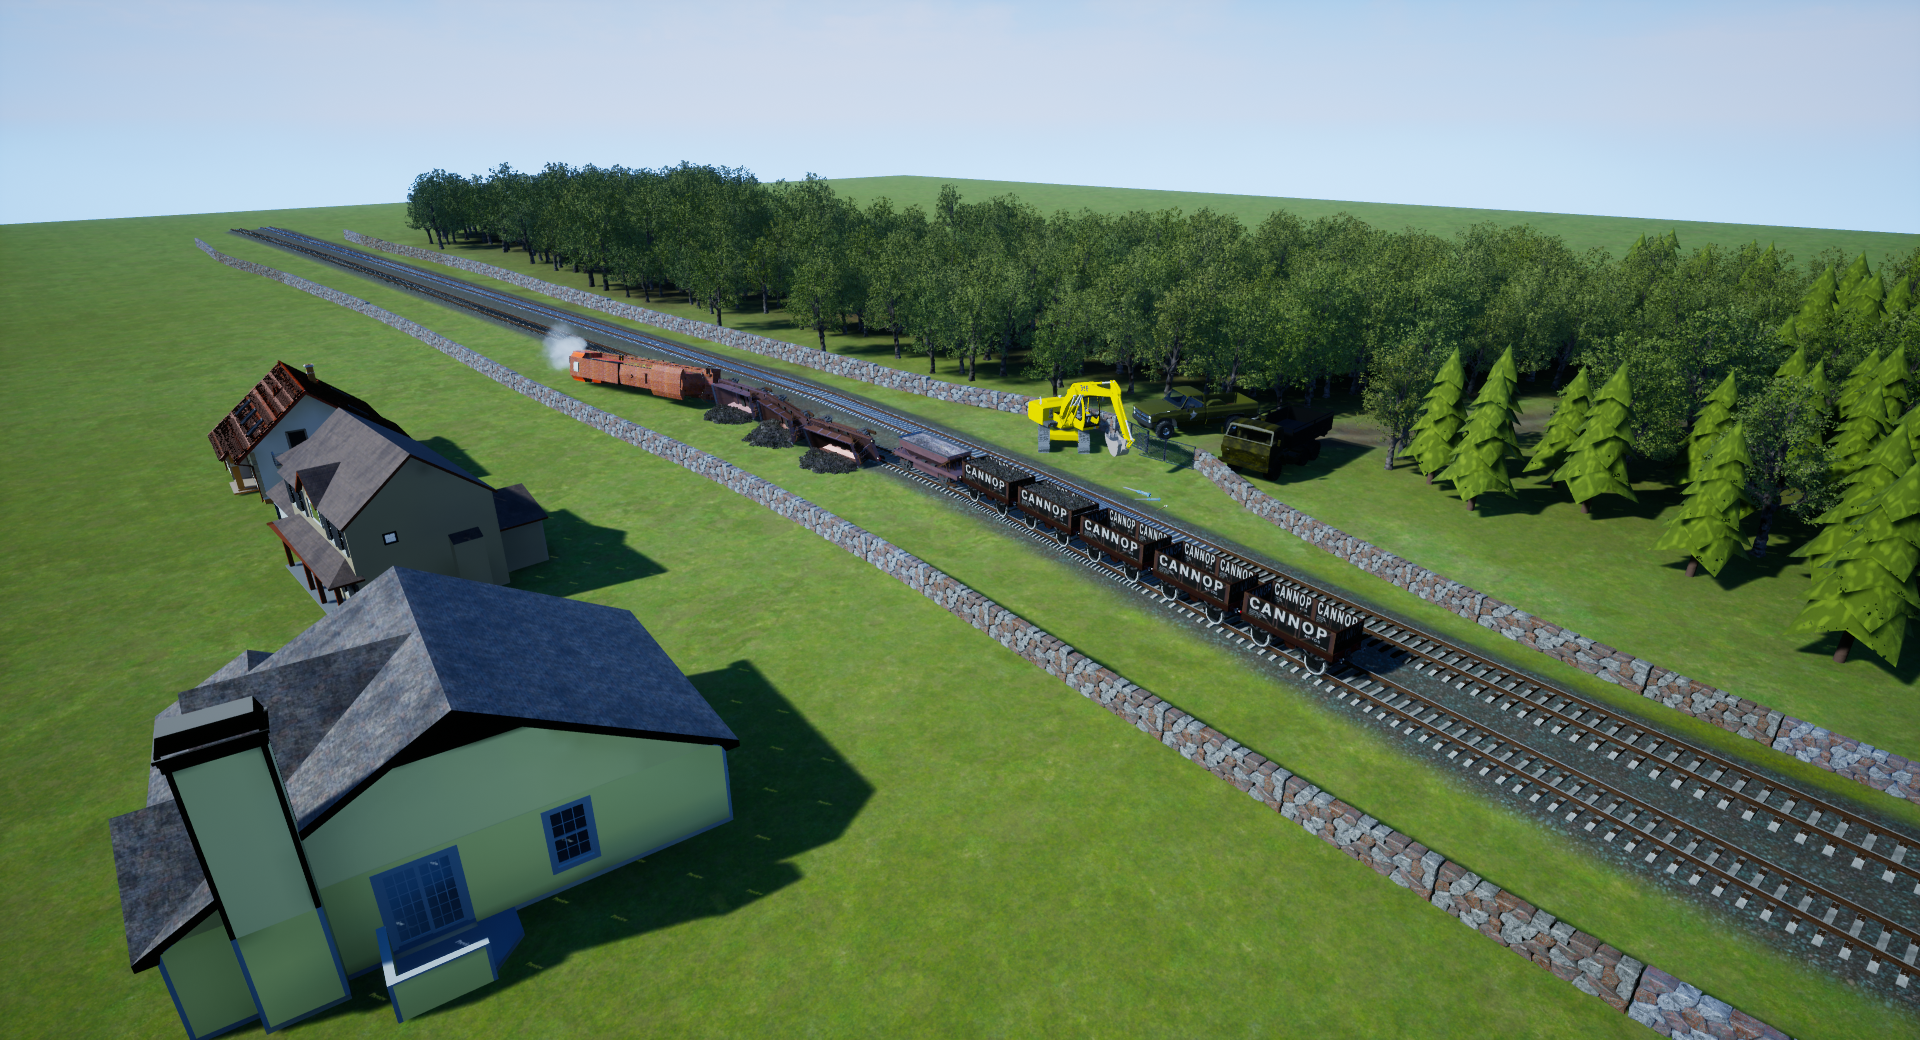
\includegraphics[width = 7cm]{Chapters/SimulationEnv/Figs/VirtualEnvV4/IsometricView2.png}} &
\subfloat{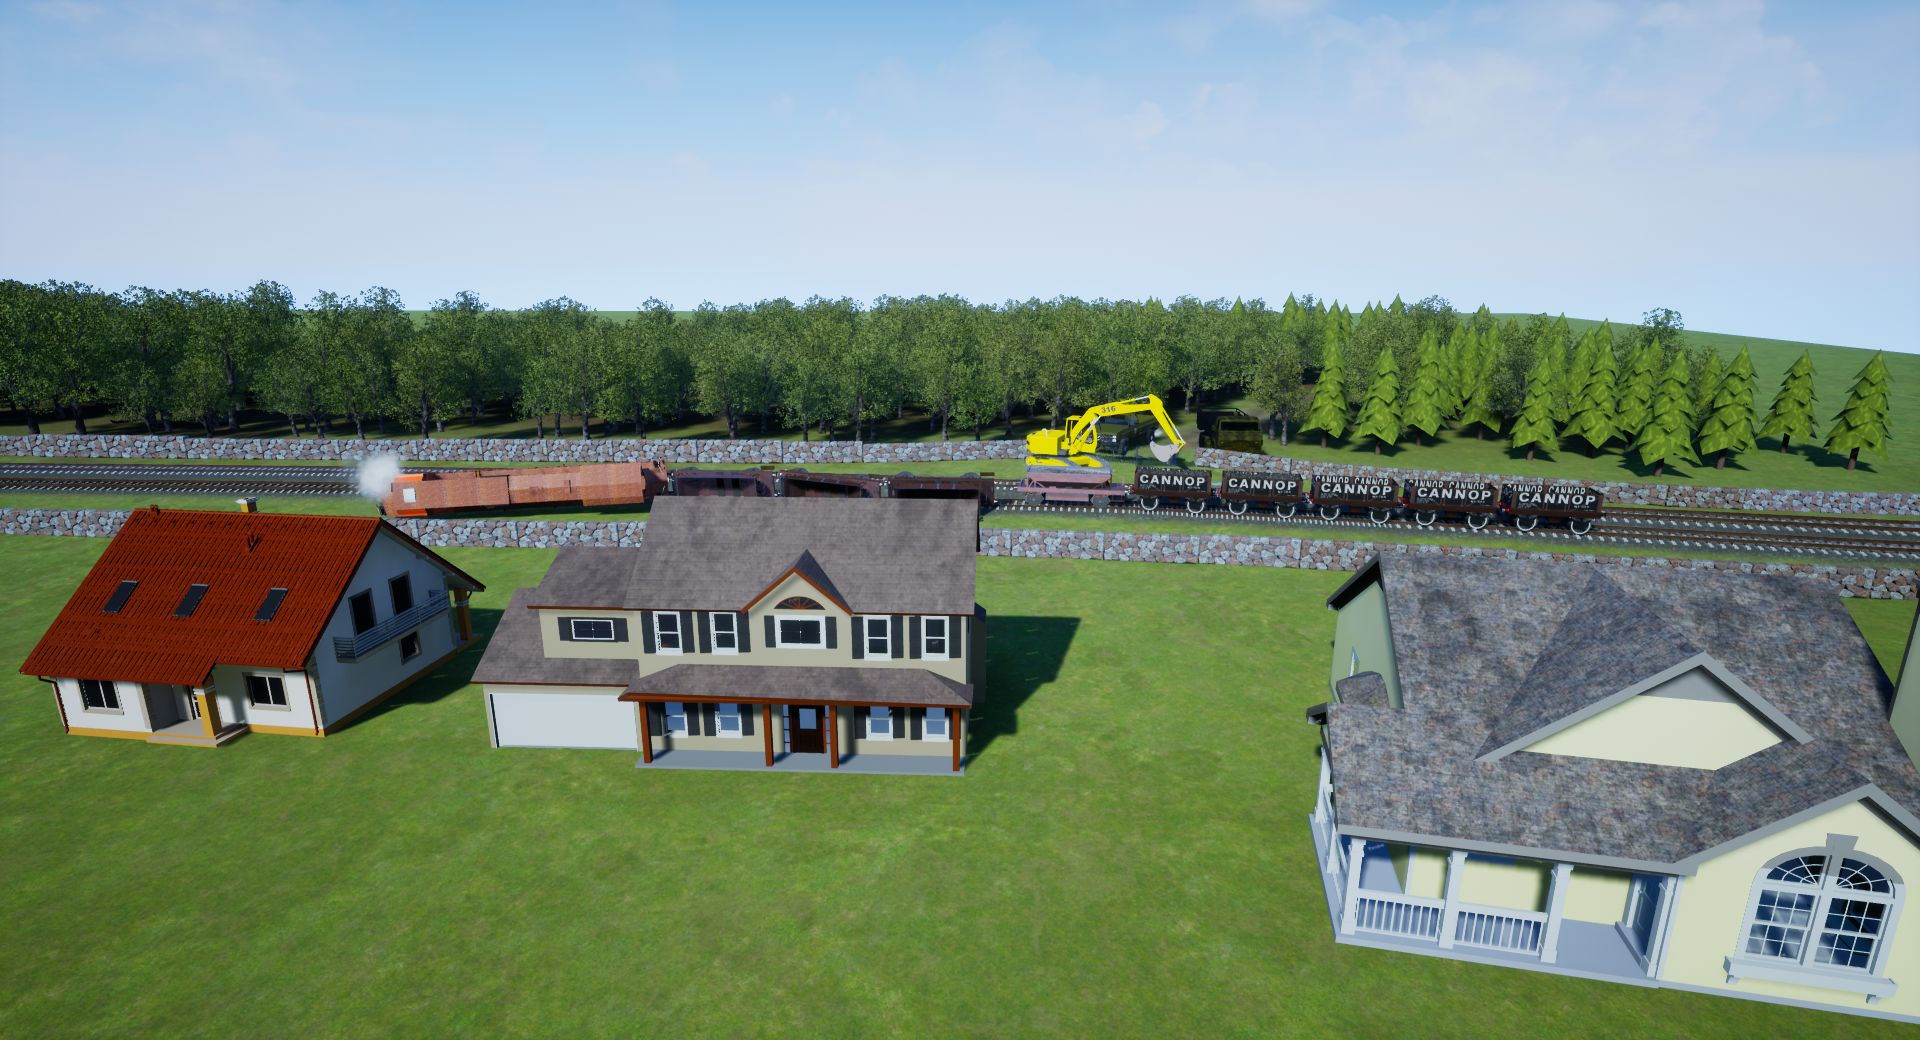
\includegraphics[width = 7cm]{Chapters/SimulationEnv/Figs/VirtualEnvV4/LowView2.png}}\\
%5thline of images
\subfloat{\includegraphics[width = 7cm]{Chapters/SimulationEnv/Figs/VirtualEnvV5/TopView.png}} &
\subfloat[Road and extra walls added]{\includegraphics[width = 7cm]{Chapters/SimulationEnv/Figs/VirtualEnvV5/IsometricView.png}} &
\subfloat{\includegraphics[width = 7cm]{Chapters/SimulationEnv/Figs/VirtualEnvV5/LowView.png}}
\end{tabular}
\caption{Evolution of the Simulation Environment. Each row depicts images from a subsequent iteration of the environment.}
\label{fig:virutalEnvDevelopment2}
\end{figure}
%\captionsetup[subfigure]{labelformat=default}
\end{landscape}



%\note{Might not be necessary to talk about all of these things}

\begin{landscape}
\begin{figure}
\centering
\begin{tabular}{cc}
\subfloat{\includegraphics[width = 10.7cm]{Chapters/SimulationEnv/Figs/VirtualEnvFinal/IsometricView1.png}} &
\subfloat{\includegraphics[width = 10.7cm]{Chapters/SimulationEnv/Figs/VirtualEnvFinal/LowView.png}} \\

\subfloat{\includegraphics[width = 10.7cm]{Chapters/SimulationEnv/Figs/VirtualEnvFinal/TopView2.png}} &
\subfloat{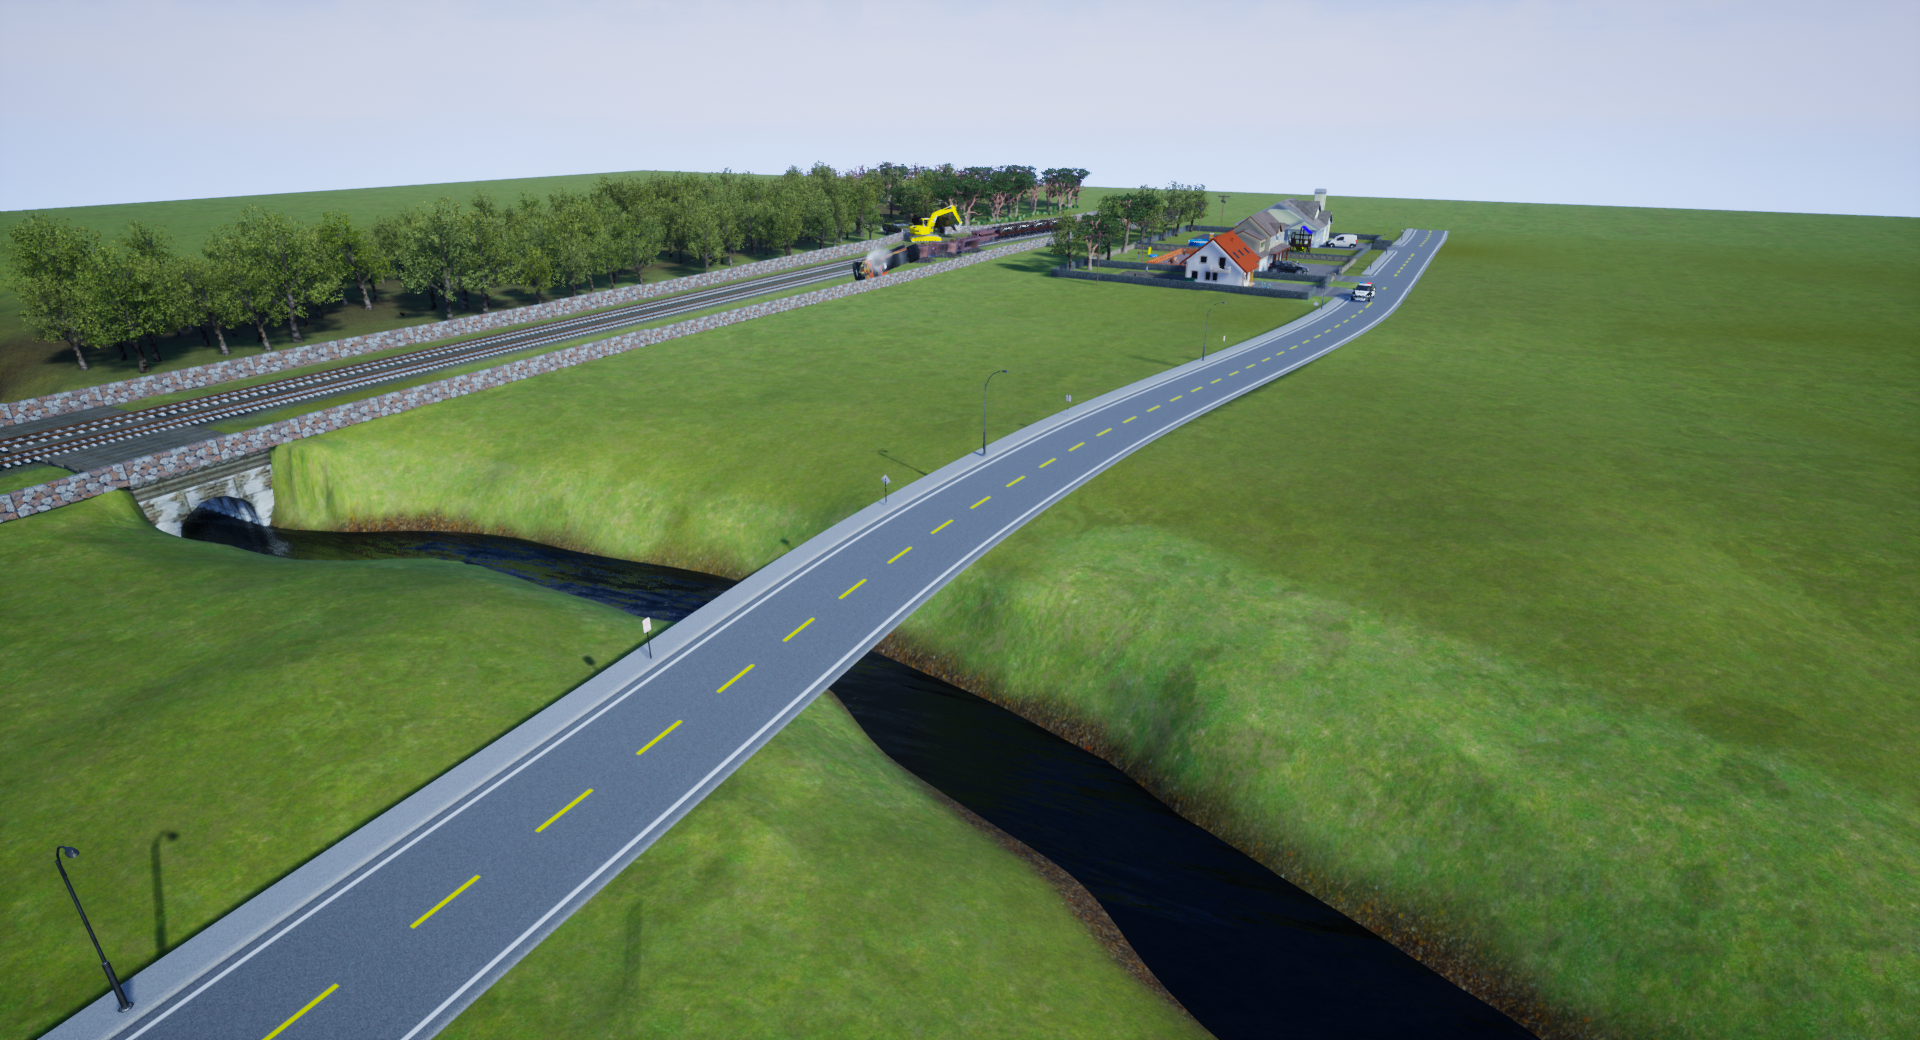
\includegraphics[width = 10.7cm]{Chapters/SimulationEnv/Figs/VirtualEnvFinal/BridgeView1.png}} \\
\end{tabular}
\caption{Images From Final Version of Simulation Environment}
\label{fig:finalVirtualEnv1}
\end{figure}


\begin{figure}
\begin{tabular}{cc}
\subfloat{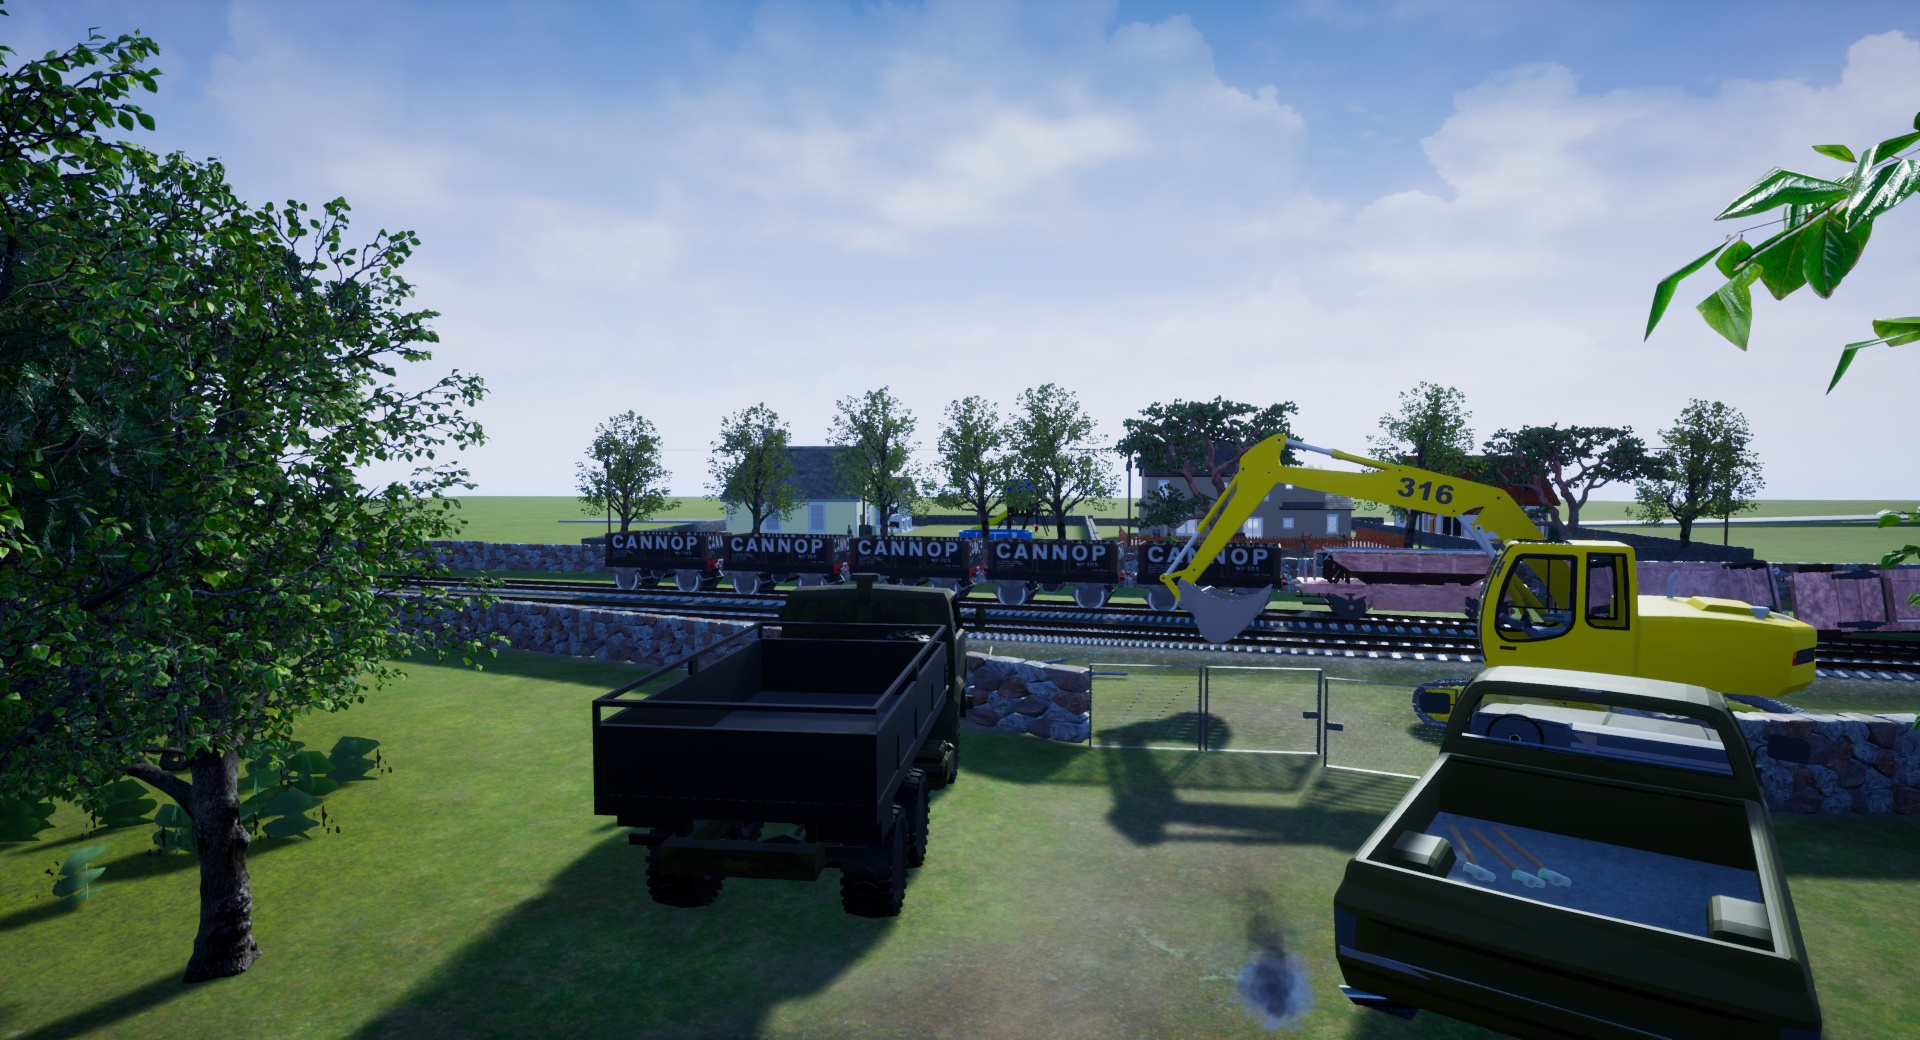
\includegraphics[width = 10.7cm]{Chapters/SimulationEnv/Figs/VirtualEnvFinal/CloseUp1.png}} &
\subfloat{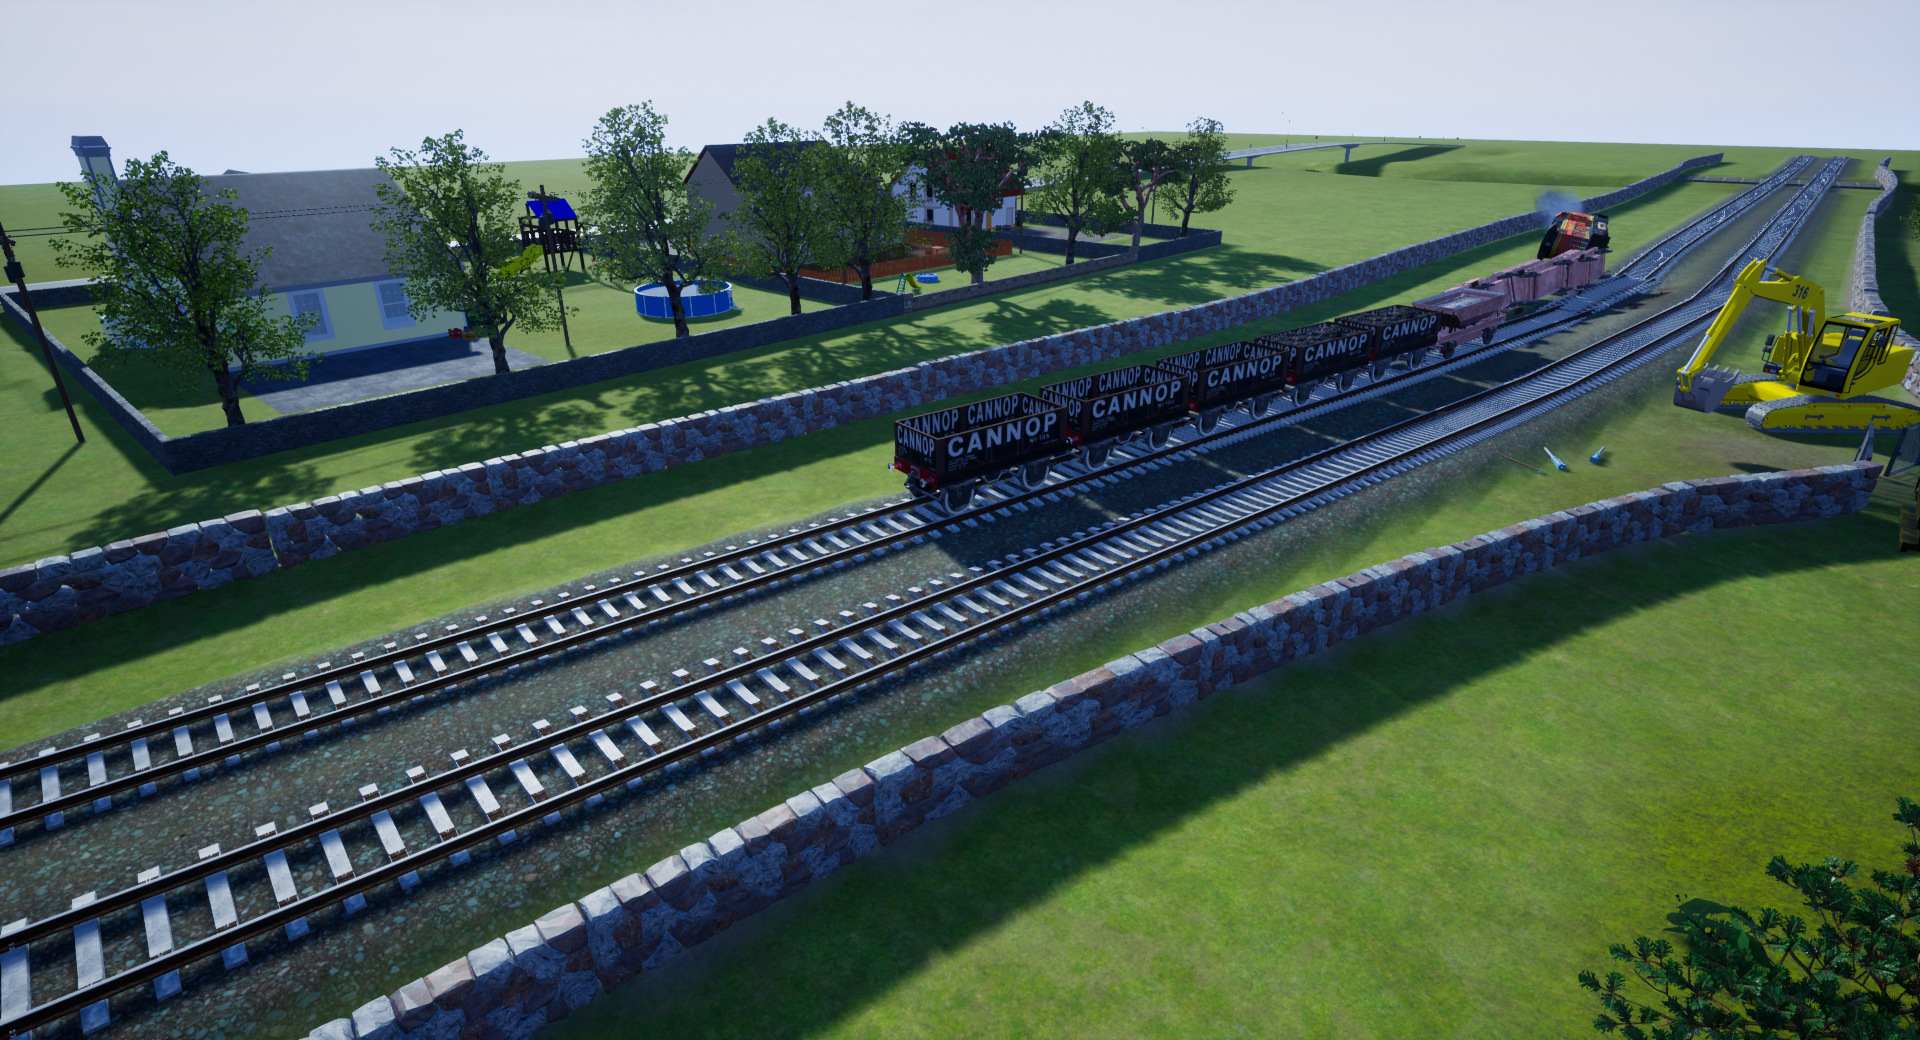
\includegraphics[width = 10.7cm]{Chapters/SimulationEnv/Figs/VirtualEnvFinal/CloseUp2.png}}
\end{tabular}
\caption{Images From Final Version of Simulation Environment}
\label{fig:finalVirtualEnv2}
\end{figure}
\end{landscape}
\pagebreak


\subsection{Techniques used to Improve Realism}\label{subsec:TechniquesImproveRealism}
\subsubsection{Blueprint Visual Scripting System}\label{subsubsec:blueprints}
UE4 uses a visual scripting system to provide a lot of functionality, known as \textit{Blueprints}. We provide a brief summary of Blueprints based on the UE4 
\href{https://docs.unrealengine.com/en-US/Engine/Blueprints/index.html}{documentation page}\footnote{\href {https://docs.unrealengine.com/en-US/Engine/Blueprints/index.html}{https://docs.unrealengine.com/en-US/Engine/Blueprints/index.html}}
. Blueprints provide a node-based interface to create gameplay elements. To develop different aspects of a game, the system provides a visual approach to scripting, and many of the tools available in standard written scripting languages are available, such as typed variables, arrays, structs, loops, etc. Blueprints were used extensively to develop the simulation.
%https://docs.unrealengine.com/en-US/Engine/Blueprints/index.html

\subsubsection{Materials}
%\note{grass, rail tracks}

%\subfloat[caption]{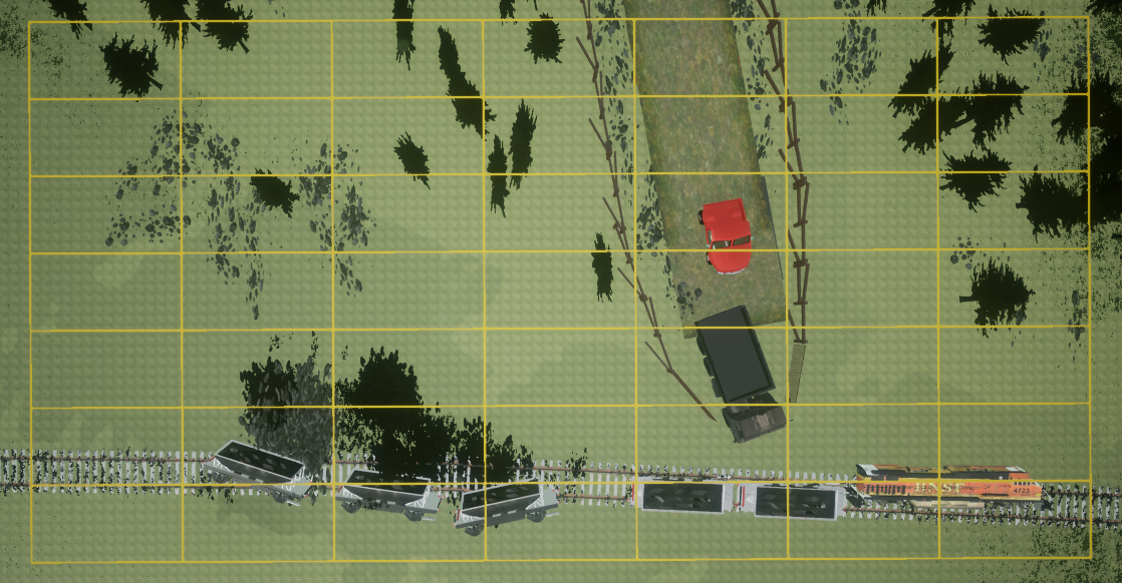
\includegraphics[width = 4.5cm]{Chapters/SimulationEnv/Figs/RailScenarioFirstIteration.png}} &
%\subfloat[caption]{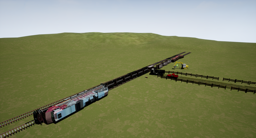
\includegraphics[width = 4.5cm]{Chapters/SimulationEnv/Figs/VirtualEnvV1/resized_HighresScreenshot00001.png}} \\

\begin{wrapfigure}{r}{0.65\textwidth}
    \centering
    \includegraphics[width=0.65\textwidth]{Chapters/SimulationEnv/Figs/BlendedMaterialsVSNotBlendedMaterials/PoorTextures.png}
    \caption{Materials used in the first iteration}
    \label{fig:PoorTextures}
    \includegraphics[width=0.65\textwidth]{Chapters/SimulationEnv/Figs/BlendedMaterialsVSNotBlendedMaterials/HighQualityMaterial.png}
    \caption{Materials used in the final iteration}
    \label{fig:GoodTextures}
    %\caption{Contrast between initial and final materials used in simulation environment.}
\end{wrapfigure}

%https://docs.unrealengine.com/en-US/Engine/Rendering/Materials/IntroductionToMaterials/index.html
The details of creating materials can be found in the 
\href{https://docs.unrealengine.com/en-US/Engine/Rendering/Materials/IntroductionToMaterials/index.html}{UE4 Documentation}\footnote{\href {https://docs.unrealengine.com/en-US/Engine/Rendering/Materials/IntroductionToMaterials/index.html}{https://docs.unrealengine.com/en-US/Engine/Rendering/Materials/IntroductionToMaterials/index.html}}, which we use as a reference for the following paragraph.
Materials are made up of a number of components in UE4, which specify aspects such as colour, opacity, roughness, specularity and emissive colours. In order to produce realistic materials, it is necessary to blend and layer different textures as well as identifying the correct parameters for surface normals and specularity, among the other features. The UE4 editor is equipped with tools for modifying materials to achieve a high-fidelity output, which we accessed through the Blueprints interface. The landscape in the first iteration of the virtual environment consisted of a single uniform texture, with none of the above parameters specified. The result is shown in Figure \ref{fig:PoorTextures}. Subsequent versions used multiple layers and blending in order to create a higher-fidelity material, with relevant parameters tuned. The final version is shown in Figure \ref{fig:GoodTextures}. Figure \ref{fig:LandscapeMaterialBlueprint} shows how a Blueprint was used to create the landscape material, where a Landscape Layer Blend node is used to combine individual textures to create the material.

\begin{figure}
\centering
\begin{tabular}{cc}
\subfloat[Layers blended into Landscape Layer Blend Node \label{fig:MaterialLayerBlend}]{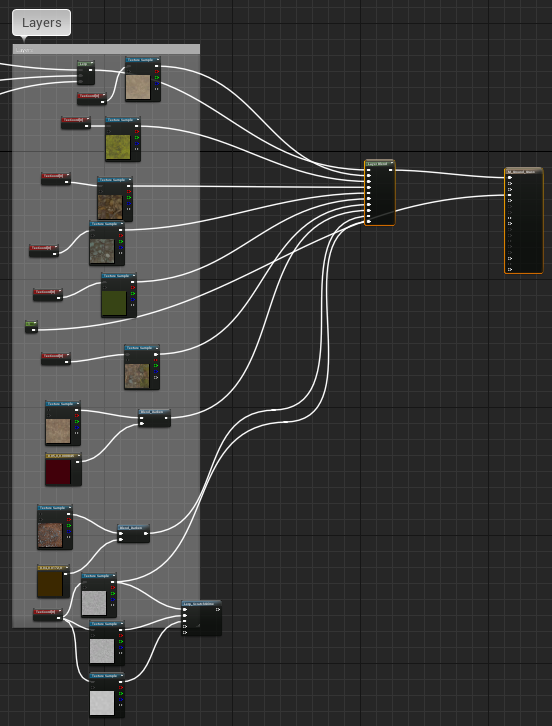
\includegraphics[width=6cm]{Chapters/SimulationEnv/Figs/BlendedMaterialsVSNotBlendedMaterials/LayerBlend.PNG}} &


\subfloat[Blueprint used to create landscape material\label{fig:MaterialBlueprint}]{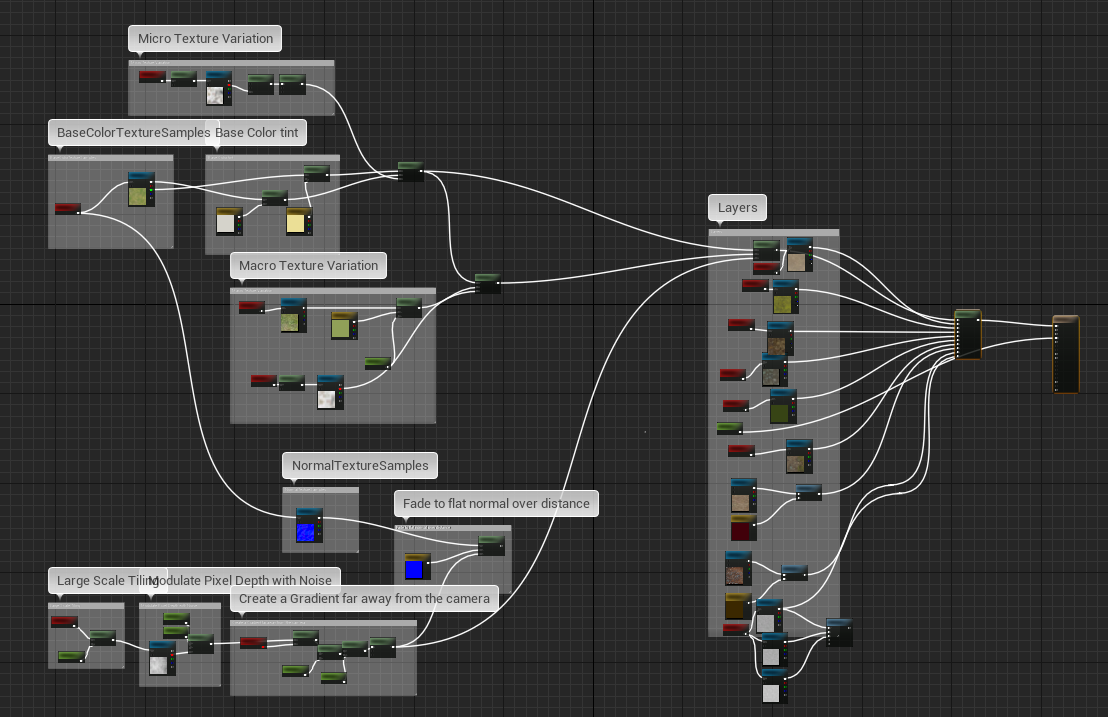
\includegraphics[width=8.5cm]{Chapters/SimulationEnv/Figs/BlendedMaterialsVSNotBlendedMaterials/LandscapeMaterial.PNG}}
\end{tabular}
\caption{Blueprints used to create the landscape}
\label{fig:LandscapeMaterialBlueprint}
\end{figure}

\pagebreak

\subsubsection{Splines}

\begin{wrapfigure}{r}{0.65\textwidth}
    \centering
    \includegraphics[width=0.65\textwidth]{Chapters/SimulationEnv/Figs/SplineVSNoSplineExamples/PerfectlyStraightRail.png}
    \caption{Non-Splined rail section in first environment iteration}
    \label{fig:StraightRail}
    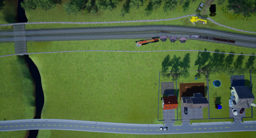
\includegraphics[width=0.65\textwidth]{Chapters/SimulationEnv/Figs/SplineVSNoSplineExamples/resized_SplineExample1.png}
    \caption{Splined rail section in final environment iteration}\label{fig:SplinedRail}
    
\end{wrapfigure}

Uniformity tends to be rare in the real world; perfectly straight lines do not occur naturally often. For this reason UE4 offers tools to create splines, along which the terrain can be deformed. We base our explanation on the official \href{https://docs.unrealengine.com/en-US/Engine/BlueprintSplines/index.html}{documentation page}\footnote{\href {https://docs.unrealengine.com/en-US/Engine/BlueprintSplines/index.html}{https://docs.unrealengine.com/en-US/Engine/BlueprintSplines/index.html}}. Splines are typically used to model roads and paths, but the Landscape Spline system is very flexible and can be used to model many different phenomena. In the initial stages of the simulation environment, only a perfectly straight section of rail could be sourced for use in the environment, as shown in Figure \ref{fig:StraightRail}. The spline tool allowed for much more realistic construction of the section of rail and accompanying wall, as shown in Figure \ref{fig:SplinedRail}. It was also used to create the road and the bridge. %\note{maybe provide link to docs}
%

\subsubsection{Foliage}
Similar to the argument made in relation to splines, it is rare to have uniformly configured foliage in the real world. In order to address this, there exist foliage generation and editing tools in UE4 editor. Version 4.18 of the editor onward contains the \href{https://docs.unrealengine.com/en-US/Engine/OpenWorldTools/ProceduralFoliage/QuickStart/index.html}{Procedural Foliage Tool}\footnote{\href {https://docs.unrealengine.com/en-US/Engine/OpenWorldTools/ProceduralFoliage/QuickStart/index.html}{https://docs.unrealengine.com/en-US/Engine/OpenWorldTools/ProceduralFoliage/QuickStart/index.html}}, 
which is the most convenient way to add swathes of foliage to a scene. Since we were using other content dependent on UE 4.16, we opted to use the foliage painter tool, which allows the user to effectively paint foliage directly onto a landscape. It allows the user to specify a number of parameters to achieve the required density, scaling and other relevant features. The results of applying foliage to the scene are visible in Figures \ref{fig:Foliage3}, \ref{fig:Foliage4} and \ref{fig:Foliage5}.
%\begin{landscape}
%\begin{figure}
%\centering
%\begin{tabular}{ccc} 
%\subfloat[Layers blended into Landscape Layer Blend Node]{\includegraphics[width=7cm]{Chapters/SimulationEnv/Figs/Foliage/Foliage2.png}}\label{fig:Foliage3} &

%\subfloat[Blueprint used to create landscape material]{\includegraphics[width=7cm]{Chapters/SimulationEnv/Figs/Foliage/Foliage5.png}}\label{fig:Foliage4} &
%\subfloat[Blueprint used to create landscape material]{\includegraphics[width=7cm]{Chapters/SimulationEnv/Figs/Foliage/Foliage6.png}}\label{fig:Foliage5}
%\end{tabular}
%\caption{Blueprints used to create realistic foliage}
%\label{fig:RealisticFoliageBlueprints}
%\end{figure}
\begin{figure}[H]
\centering
\begin{tabular}{c} 
\subfloat[Layers blended into Landscape Layer Blend Node \label{fig:Foliage3}]{\includegraphics[width=12cm]{Chapters/SimulationEnv/Figs/Foliage/Foliage2.png}} \\

\subfloat[Trees and shrubs generated with non-uniform configuration \label{fig:Foliage4} ]{\includegraphics[width=12cm]{Chapters/SimulationEnv/Figs/Foliage/Foliage5.png}}\\

%--------- This breaks the page and begins the last figure on a new page ---------%
\end{tabular}
\caption{Examples of foliage in the simulation environment}
\end{figure}
\clearpage
\begin{figure}[H]
\ContinuedFloat
\centering
\begin{tabular}{c}
%--------- This breaks the page and begins the last figure on a new page ---------%

\subfloat[Woodland area effect \label{fig:Foliage5}]{\includegraphics[width=12cm]{Chapters/SimulationEnv/Figs/Foliage/Foliage6.png}}
\end{tabular}
\caption{Examples of foliage in the simulation environment}
%\label{fig:RealisticFoliageBlueprints}
\end{figure}






%\begin{landscape}


%\end{landscape}

\subsubsection{Landscape Editing}
%\note{Discuss here how dirt track was created using}
%Creating a realistic landscape in UE4 serves a number of purposes. 
To realistically model the configuration of physical objects and their corresponding shadow and occlusion effects, it was necessary to model the terrain realistically. This was also desirable to allow the potential simulation of ground vehicles, so that difficulties that may be experienced in the real world, such as steep climbs or highly uneven surfaces, may be taken into account. UE4 provides a suite of landscaping tools that allows the user to create a highly variable landscape. The tools facilitate raising and flattening, smoothing, random noise and simulated erosion, as well as allowing for other more detailed modifications. These were used to create the railway embankment, the rutted path leading onto the rail tracks and the riverbank and riverbed, shown in Figure \ref{fig:LandscapeEditing}.

\begin{figure}[H]
\centering
\begin{tabular}{c}
\subfloat[Rutted Track]{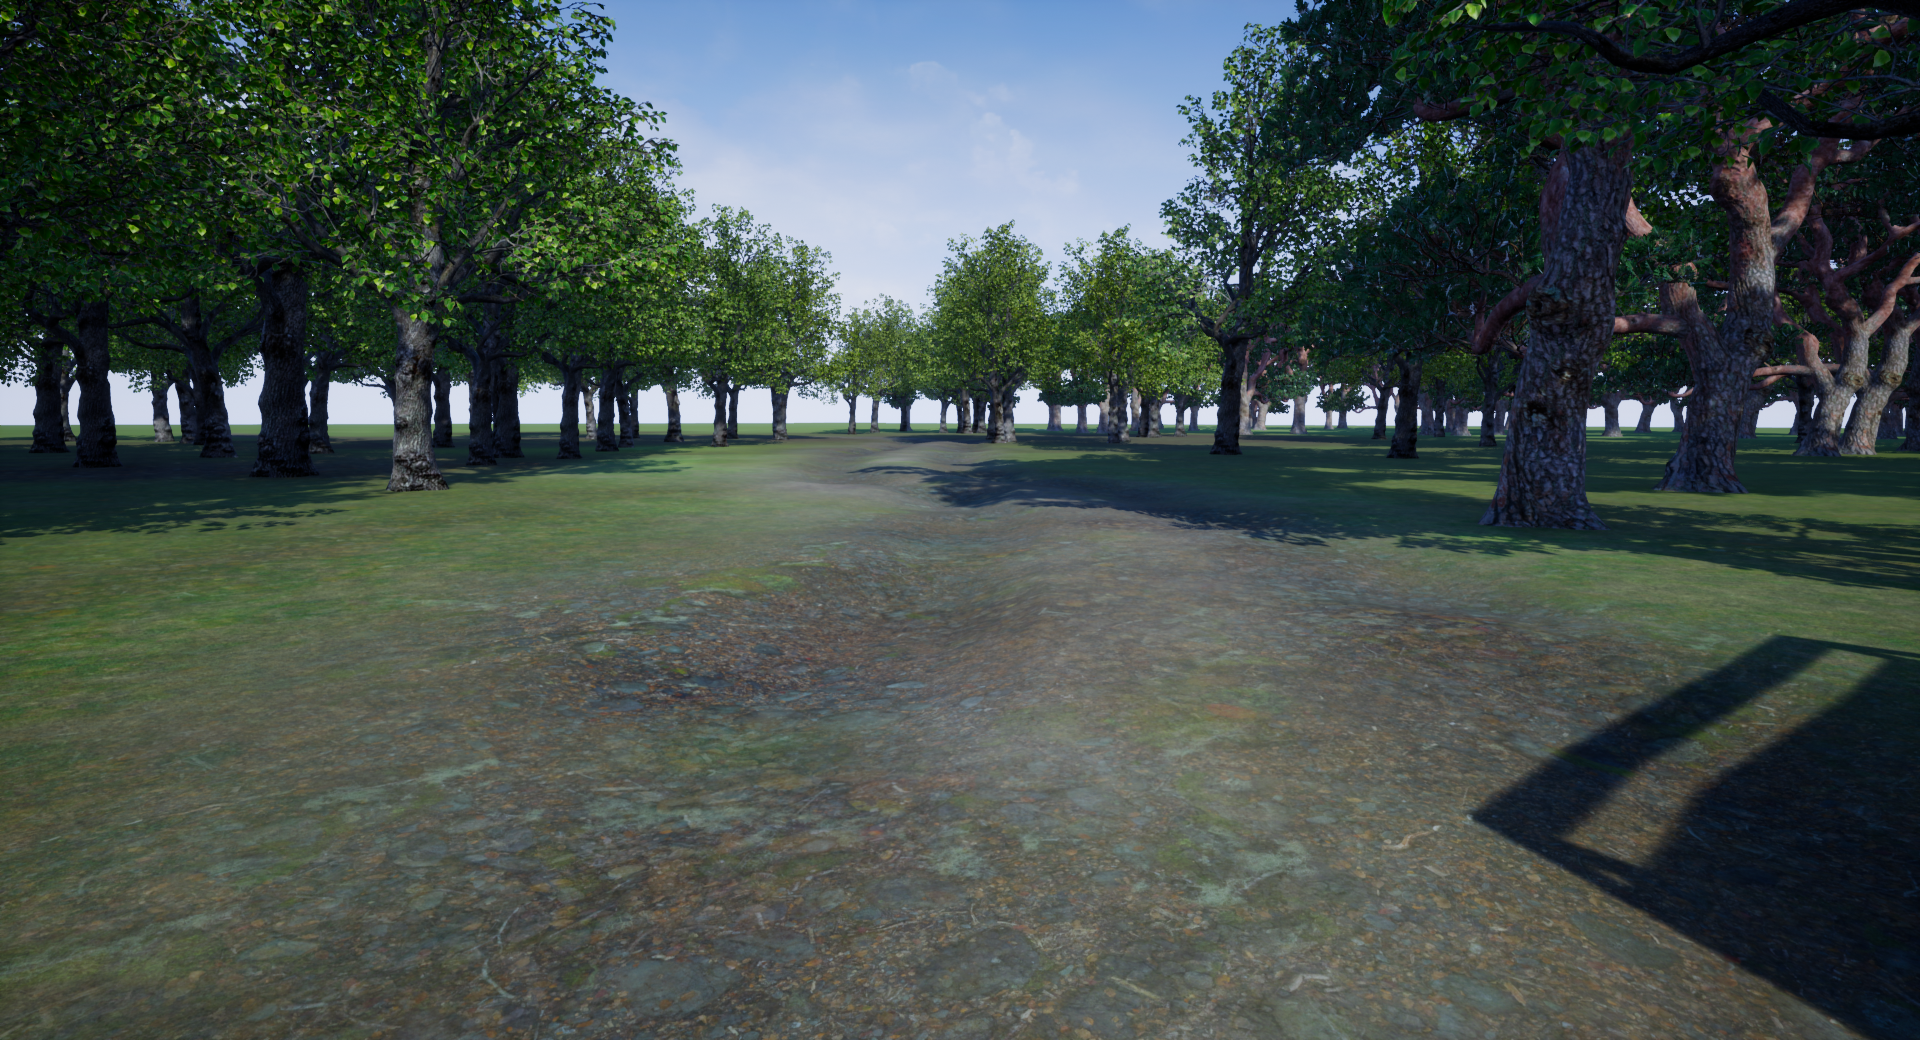
\includegraphics[width=11.6cm]{Chapters/SimulationEnv/Figs/LandscapedVSNotLandscaped/RuttedTrack.png}}\label{fig:RuttedTrack} \\
\subfloat[Rail embankment]{\includegraphics[width=11.6cm]{Chapters/SimulationEnv/Figs/LandscapedVSNotLandscaped/RailwayEmbankment.png}}\label{fig:RailEmbankment} \\

%\end{tabular}
%\end{figure}
%\clearpage
%\begin{figure}[H]
%\ContinuedFloat
%\centering
%\begin{tabular}{c}

\subfloat[Riverbank]{\includegraphics[width=11.6cm]{Chapters/SimulationEnv/Figs/LandscapedVSNotLandscaped/Bridge.png}}\label{fig:Riverbank}

\end{tabular}
\caption{Results of using the UE4 landscape editing tools}
\label{fig:LandscapeEditing}
\end{figure}


\subsubsection{Asset Sourcing}
%
An \href{https://docs.unrealengine.com/en-US/Engine/Basics/AssetsAndPackages/index.html}{\textit{asset}}\footnote{\href{https://docs.unrealengine.com/en-US/Engine/Basics/AssetsAndPackages/index.html}{https://docs.unrealengine.com/en-US/Engine/Basics/AssetsAndPackages/index.html}} can be described as a piece of content for an Unreal Engine project, which has been serialized to a file. Assets can be re-used and modified in the UE4 editor, but are usually created using external software. UE4 uses assets that come in the Filmbox (.fbx) format, which is a proprietary file format owned by Autodesk.
%\note{Do I need to reference this?}. Conversion tools do exist from other common asset file formats to fbx, but results can vary. Due to limited funding, time and experience, we decided to avoid creating assets from scratch but rather used assets that were free to use. Searching for free assets is a labor-intensive process, as it consisted of a number of steps:
\begin{enumerate}
    \item First, identify possible candidates for a particular type of asset (e.g. a train) based on a search of asset stores that offer free assets. We mainly used \href{https://www.cgtrader.com/}{CGTrader}\footnote{\href {https://www.cgtrader.com/}{https://www.cgtrader.com/}} ,
    
    \href{https://www.turbosquid.com/}{TurboSquid}\footnote{\href {https://www.turbosquid.com/}{https://www.turbosquid.com/}}
    , 
    \href{https://3dwarehouse.sketchup.com/?hl=en}{3D Warehouse}\footnote{\href {https://3dwarehouse.sketchup.com/?hl=en}{https://3dwarehouse.sketchup.com/?hl=en}} 
    and
    \href{https://www.shapenet.org/}{ShapeNet}\footnote{\href {https://www.shapenet.org/}{https://www.shapenet.org/}}.
    
    \item Once a potentially suitable asset had been identified based on its description and preview, it was downloaded in the Filmbox (fbx) format if possible. Otherwise, it was downloaded in whatever format was available. 
    \item The asset was opened in Autodesk \note{add reference} and visually inspected for suitability. If the textures and geometry were not of a sufficient standard the processes was restarted.
    \item If the asset was deemed suitable from the inspection in Autodesk, then it was exported in Filmbox format.
    \item The asset was then imported into the UE4 editor. Problems often arose in scaling, incorrect texture mapping and one-sided materials applied to the wrong side of assets. These problems could sometimes be addressed; if not we had to restart the process.
\end{enumerate}

%Talk about how well static world matches specification, how well rendered images perform for training some object detection etc.
%Also talk about how the environment was packaged and open-sourced with permissive licence for general use



% Not sure of exact ordering here
% 1st Iteration J:\Work\David\ROCSAFEMidTermDemo\Code\UnrealEngine\AirSim\Unreal\Environments\Blocks
% 2nd Iteration J:\Work\David\UnrealEngineRocsafe\OS_01RadIntegr
% 3rd Iteration D:\ROCSAFEScenarios\OS01TestTemp
% 4th Iteration D:\ROCSAFEScenarios\OS_01Radiation - D:\ROCSAFEScenarios\OS_01Radiation\Saved\Screenshots\Windows screenshot 11
% 5th \\ROCSAFE2\ROCSAFEGroupShared\ROCSAFEUnrealEngineOperatingScenarios\NotIntegratedAirSim

% V1: Brussels Demo
% V2: Rail with spline, train, digger. No dirt track, no houses, no road, no wall, poor textures, poor foliage
% V3: Add wall, better foliage
% V4:and houses
% V5: Proper foliage (stones) & blended textures
% V6: Final version in shared folder
